\section{Рабочий проект}

\subsection{Спецификация классов программной системы}

В данном разделе приведено описание основных классов и модулей, разработанных в процессе реализации веб-приложения «Цифровая платформа Курский край». Для каждого класса указаны его назначение, а также перечень методов с модификаторами доступа и кратким описанием. Для модулей, состоящих из набора функций, приводится описание каждой функции.

\subsubsection{Модуль places-store (центральное хранилище данных)}

Модуль \texttt{places-store.js} предназначен для управления данными о местах, категориях и маршрутах. Он инкапсулирует HTTP-вызовы к REST API, выполняет нормализацию и валидацию данных, а также предоставляет методы для CRUD-операций. Функции модуля \texttt{places-store.js} приведены в таблице~\ref{tab:placesstorage}.

\begin{xltabular}{\textwidth}{|X|c|X|}
	\caption{Функции модуля \texttt{places-store.js}}
	\label{tab:placesstorage}\\
	\hline
	Функция & Доступ & Описание \\
	\hline
	\endfirsthead
	\caption*{Продолжение таблицы~\ref{tab:placesstorage}}\\
	\hline
	Функция & Доступ & Описание \\
	\hline
	\finishhead
	\texttt{normalizePlace(raw)} & public & Приводит сырые данные места к единому формату (типы, значения по умолчанию). \\ \hline
	\texttt{validatePlace(place)} & public & Проверяет корректность объекта места (обязательные поля, типы). \\ \hline
	\texttt{loadPlaces()} & public & Загружает список опубликованных мест через API. \\ \hline
	\texttt{getAdminPlaces()} & public & Загружает все места (включая скрытые) для админ-панели. \\ \hline
	\texttt{savePlace(place)} & public & Сохраняет (создаёт или обновляет) место через POST /api/places. \\ \hline
	\texttt{deletePlace(id)} & public & Удаляет место через DELETE /api/places/:id. \\ \hline
	\texttt{getCategories()} & public & Возвращает список категорий (из API или встроенного справочника). \\ \hline
	\texttt{addCategory(label)} & public & Добавляет новую категорию через POST /api/categories. \\ \hline
	\texttt{normalizeRoute(raw)} & public & Приводит сырые данные маршрута к единому формату. \\ \hline
	\texttt{validateRoute(route)} & public & Проверяет корректность маршрута (наличие названия, минимум 2 точки). \\ \hline
	\texttt{loadRoutes()} & public & Загружает список опубликованных маршрутов с точками. \\ \hline
	\texttt{getAdminRoutes()} & public & Загружает все маршруты (включая скрытые) для админ-панели. \\ \hline
	\texttt{saveRoute(route)} & public & Сохраняет маршрут транзакционно (POST /api/routes). \\ \hline
	\texttt{deleteRoute(id)} & public & Удаляет маршрут через DELETE /api/routes/:id. \\ \hline
\end{xltabular}

\subsubsection{Модуль map-init (управление картой)}

Модуль \texttt{map-init.js} содержит набор функций для инициализации карты Yandex, добавления маркеров, обработки кликов и взаимодействия с модальными окнами. Функции модуля \texttt{map-init.js} приведены в таблице~\ref{tab:mapinit}.

\begin{xltabular}{\textwidth}{|X|c|X|}
	\caption{Функции модуля \texttt{map-init.js}}
	\label{tab:mapinit}\\
	\hline
	Функция & Доступ & Описание \\
	\hline
	\endfirsthead
	\caption*{Продолжение таблицы~\ref{tab:mapinit}}\\
	\hline
	Функция & Доступ & Описание \\
	\hline
	\finishhead
	\texttt{initMap()} & internal & Выполняет асинхронную загрузку мест, создаёт карту, добавляет маркеры, устанавливает границы. \\ \hline
	\texttt{buildPlacemark(place)} & internal & Создаёт объект \texttt{ymaps.Placemark} для одного места с иконкой по категории. \\ \hline
	\texttt{openMapModal(place)} & internal & Открывает модальное окно с краткой информацией о месте. \\ \hline
	\texttt{setActiveById(id)} & public & Центрирует карту на указанном месте и открывает его карточку. \\ \hline
	\texttt{bindModalClose()} & internal & Назначает обработчики закрытия модального окна (клик вне, Escape). \\ \hline
	\texttt{scrollToMap()} & internal & Плавно прокручивает страницу к блоку карты. \\ \hline
\end{xltabular}

\subsubsection{Модуль admin-page (административный интерфейс)}

Модуль \texttt{admin-page.js} реализует всю логику административной панели: отображение списков объектов и маршрутов, формы добавления/редактирования, выбор координат на карте, управление точками маршрута. Функции модуля \texttt{admin-page.js} приведены в таблице~\ref{tab:adminpage}.

\begin{xltabular}{\textwidth}{|X|c|X|}
	\caption{Функции модуля \texttt{admin-page.js}}
	\label{tab:adminpage}\\
	\hline
	Функция & Доступ & Описание \\
	\hline
	\endfirsthead
	\caption*{Продолжение таблицы~\ref{tab:adminpage}}\\
	\hline
	Функция & Доступ & Описание \\
	\hline
	\finishhead
	\texttt{fillCategorySelect()} & internal & Заполняет выпадающий список категорий в форме объекта. \\ \hline
	\texttt{readForm()} & internal & Считывает данные из формы объекта и возвращает нормализованный объект. \\ \hline
	\texttt{renderList()} & internal & Отображает таблицу всех мест (с кнопками редактирования/удаления). \\ \hline
	\texttt{handleSave(e)} & internal & Обработчик сохранения объекта (валидация, вызов PlacesStore.savePlace). \\ \hline
	\texttt{bindCategoryAdd()} & internal & Привязывает обработчик кнопки добавления новой категории. \\ \hline
	\texttt{renderRoutesList()} & internal & Отображает таблицу маршрутов. \\ \hline
	\texttt{handleRouteSave(e)} & internal & Обработчик сохранения маршрута (валидация, транзакционное сохранение). \\ \hline
	\texttt{renderRoutePointsList()} & internal & Отрисовывает список точек маршрута с кнопками перемещения/удаления. \\ \hline
	\texttt{initCoordsMap()} & internal & Инициализирует карту для выбора координат в модальном окне. \\ \hline
	\texttt{showCoordsModal()}, \texttt{closeCoordsModal()} & internal & Открывает/закрывает модальное окно выбора координат. \\ \hline
\end{xltabular}

\subsubsection{Модуль routes-page (отображение маршрутов)}

Модуль \texttt{routes-page.js} отвечает за пользовательскую страницу маршрутов: загрузку маршрутов, отображение карточек, построение маршрута на карте через мультимаршрутизатор Yandex. Функции модуля \texttt{routes-page.js} приведены в таблице~\ref{tab:routespage}.

\begin{xltabular}{\textwidth}{|X|c|X|}
	\caption{Функции модуля \texttt{routes-page.js}}
	\label{tab:routespage}\\
	\hline
	Функция & Доступ & Описание \\
	\hline
	\endfirsthead
	\caption*{Продолжение таблицы~\ref{tab:routespage}}\\
	\hline
	Функция & Доступ & Описание \\
	\hline
	\finishhead
	\texttt{renderRoutes(routes)} & internal & Отрисовывает список карточек маршрутов на странице. \\ \hline
	\texttt{openRouteModal(route)} & internal & Открывает модальное окно с описанием маршрута, списком точек и картой. \\ \hline
	\texttt{drawRoute(points)} & internal & Строит пешеходный маршрут по координатам точек через \texttt{ymaps.multiRouter}. \\ \hline
	\texttt{destroyRouteMap()} & internal & Уничтожает предыдущий экземпляр карты маршрута. \\ \hline
\end{xltabular}

\subsubsection{Модуль places-page (каталог мест)}

Модуль \texttt{places-page.js} реализует страницу «Куда пойти»: загрузку мест, фильтрацию по категориям, отображение карточек и модальное окно с подробной информацией. Функции модуля \texttt{places-page.js} приведены в таблице~\ref{tab:placespage}.

\begin{xltabular}{\textwidth}{|X|c|X|}
	\caption{Функции модуля \texttt{places-page.js}}
	\label{tab:placespage}\\
	\hline
	Функция & Доступ & Описание \\
	\hline
	\endfirsthead
	\caption*{Продолжение таблицы~\ref{tab:placespage}}\\
	\hline
	Функция & Доступ & Описание \\
	\hline
	\finishhead
	\texttt{renderCards(places, onOpen)} & internal & Отрисовывает карточки мест в контейнере. \\ \hline
	\texttt{renderCategoryFilters(places, onFilter)} & internal & Создаёт кнопки фильтрации по уникальным категориям. \\ \hline
	\texttt{openModal(place)} & internal & Открывает модальное окно с подробной информацией о месте (описание, галерея, контакты). \\ \hline
	\texttt{closeModal()} & internal & Закрывает модальное окно. \\ \hline
	\texttt{init()} & internal & Инициализирует страницу: загружает места, применяет фильтры из URL, назначает обработчики. \\ \hline
\end{xltabular}

\subsubsection{Модуль photos-page (фотогалерея)}

Модуль \texttt{photos-page.js} собирает все изображения (главные фото и галереи) из всех мест и отображает их в виде сетки с возможностью увеличения и перехода к месту. Функции модуля \texttt{photos-page.js} приведены в таблице~\ref{tab:photospage}.

\begin{xltabular}{\textwidth}{|X|c|X|}
	\caption{Функции модуля \texttt{photos-page.js}}
	\label{tab:photospage}\\
	\hline
	Функция & Доступ & Описание \\
	\hline
	\endfirsthead
	\caption*{Продолжение таблицы~\ref{tab:photospage}}\\
	\hline
	Функция & Доступ & Описание \\
	\hline
	\finishhead
	\texttt{buildPhotos(places)} & internal & Проходит по всем местам и собирает уникальные URL изображений с привязкой к месту. \\ \hline
	\texttt{openPhotoModal(item)} & internal & Открывает модальное окно с увеличенным фото. \\ \hline
	\texttt{openPlaceModal(place)} & internal & Открывает модальное окно с информацией о месте, связанном с фото. \\ \hline
	\texttt{closeModal(id)} & internal & Закрывает указанное модальное окно. \\ \hline
\end{xltabular}

\subsubsection{Модуль theme (переключение темы)}

Модуль \texttt{theme.js} обеспечивает переключение между светлой и тёмной темой оформления с сохранением выбора в \texttt{localStorage}. Функции модуля \texttt{theme.js} приведены в таблице~\ref{tab:theme}.

\begin{xltabular}{\textwidth}{|X|c|X|}
	\caption{Функции модуля \texttt{theme.js}}
	\label{tab:theme}\\
	\hline
	Функция & Доступ & Описание \\
	\hline
	\endfirsthead
	\caption*{Продолжение таблицы~\ref{tab:theme}}\\
	\hline
	Функция & Доступ & Описание \\
	\hline
	\finishhead
	\texttt{setTheme(name)} & internal & Устанавливает атрибут \texttt{data-theme} на body и сохраняет в localStorage. \\ \hline
	\texttt{toggleTheme()} & public & Переключает тему (light/dark). \\ \hline
	\texttt{init()} & internal & Восстанавливает сохранённую тему, назначает обработчик кнопке. \\ \hline
\end{xltabular}

\subsubsection{Модуль ui (вспомогательные эффекты)}

Модуль \texttt{ui.js} добавляет анимацию появления при скролле, лёгкий параллакс для hero-блока и подбор случайных фотографий на главной странице. Функции модуля \texttt{ui.js} приведены в таблице~\ref{tab:ui}.

\begin{xltabular}{\textwidth}{|X|c|X|}
	\caption{Функции модуля \texttt{ui.js}}
	\label{tab:ui}\\
	\hline
	Функция & Доступ & Описание \\
	\hline
	\endfirsthead
	\caption*{Продолжение таблицы~\ref{tab:ui}}\\
	\hline
	Функция & Доступ & Описание \\
	\hline
	\finishhead
	\texttt{initAnimations()} & internal & Настраивает IntersectionObserver для элементов с атрибутом \texttt{data-anim}. \\ \hline
	\texttt{initParallax()} & internal & Добавляет эффект параллакса при скролле для hero-секции. \\ \hline
	\texttt{initHomePhotos()} & internal & Загружает случайные фотографии мест и отображает их в слайдере на главной. \\ \hline
\end{xltabular}

\subsubsection{Серверные модули (Node.js/Express)}

Серверная часть реализована в модулях \texttt{app.js} (основное приложение), \texttt{db.js} (пул соединений PostgreSQL) и \texttt{init-db.js} (инициализация схемы). В таблице приведены основные маршруты (функции-обработчики) из \texttt{app.js}. Маршруты в \texttt{app.js} приведены в таблице~\ref{tab:server}.

\begin{xltabular}{\textwidth}{|X|c|X|}
	\caption{Маршруты в \texttt{app.js}}
	\label{tab:server}\\
	\hline
	Маршрут & HTTP метод & Описание \\
	\hline
	\endfirsthead
	\caption*{Продолжение таблицы~\ref{tab:server}}\\
	\hline
	Функция (маршрут) & HTTP метод & Описание \\
	\hline
	\finishhead
	\texttt{/api/categories} & GET & Возвращает JSON-список всех категорий. \\ \hline
	\texttt{/api/categories} & POST & Создаёт или обновляет категорию (UPSERT). \\ \hline
	\texttt{/api/places} & GET & Возвращает места (с параметром \texttt{includeHidden} для админа). \\ \hline
	\texttt{/api/places} & POST & Сохраняет место (UPSERT). \\ \hline
	\texttt{/api/places/:id} & DELETE & Удаляет место по ID. \\ \hline
	\texttt{/api/routes} & GET & Возвращает маршруты с агрегированными точками. \\ \hline
	\texttt{/api/routes} & POST & Транзакционно сохраняет маршрут и его точки. \\ \hline
	\texttt{/api/routes/:id} & DELETE & Удаляет маршрут. \\ \hline
\end{xltabular}

\subsection{Системное тестирование}

Системное тестирование проводилось в соответствии со сценариями использования, определёнными в техническом задании (раздел 2.5). Для каждого сценария были разработаны тест-кейсы, содержащие описание предусловий, последовательность действий и ожидаемый результат. Тестирование выполнялось на операционной системе Windows 11 с использованием браузеров Google Chrome и Mozilla Firefox.

\subsubsection{Сводная таблица тест-кейсов}

В таблице~\ref{tab:testcases} приведён перечень всех выполненных тест-кейсов с указанием их идентификаторов и результатов.

\begin{xltabular}{\textwidth}{|c|X|c|}
	\caption{Сводная таблица тест-кейсов}
	\label{tab:testcases}\\
	\hline
	ID & Название тест-кейса & Результат \\
	\hline
	\endfirsthead
	\caption*{Продолжение таблицы~\ref{tab:testcases}}\\
	\hline
	ID & Название тест-кейса & Результат \\
	\hline
	\finishhead
	TC-01 & Отображение карты с маркерами мест & Пройден \\ \hline
	TC-02 & Фильтрация списка мест по категории & Пройден \\ \hline
	TC-03 & Открытие карточки места и просмотр галереи & Пройден \\ \hline
	TC-04 & Переход от карточки места к карте & Пройден \\ \hline
	TC-05 & Добавление нового места через админ-панель & Пройден \\ \hline
	TC-06 & Редактирование существующего места & Пройден \\ \hline
	TC-07 & Добавление новой категории & Пройден \\ \hline
	TC-08 & Создание маршрута (выбор точек, порядок) & Пройден \\ \hline
	TC-09 & Редактирование маршрута & Пройден \\ \hline
	TC-10 & Просмотр маршрута на карте (пешеходная прокладка) & Пройден \\ \hline
	TC-11 & Отображение фотогалереи всех мест & Пройден \\ \hline
	TC-12 & Выбор координат объекта на карте в админке & Пройден \\ \hline
\end{xltabular}

\subsubsection{TC-01. Отображение карты с маркерами мест}

\textbf{Предусловие:} сервер запущен, база данных заполнена тестовыми местами (минимум 3 с корректными координатами). Открыта главная страница.

\textbf{Шаги:}
\begin{enumerate}
	\item Перейти в раздел «Главная» или на страницу с картой.
	\item Дождаться загрузки Yandex Maps API.
	\item Визуально оценить наличие маркеров на карте.
	\item Навести курсор на маркер — появится подсказка с названием места.
\end{enumerate}

\textbf{Ожидаемый результат:} карта центрирована на городе Курск. На карте отображаются цветные маркеры, соответствующие категориям мест. Количество маркеров равно количеству опубликованных мест.

\textbf{Фактический результат:} пройден. Результат тестирования представ-
лен на рисунке~\ref{fig:ts-01}.

% Место для рисунка: скриншот главной страницы с картой и маркерами

\begin{figure}[H]
	\centering
	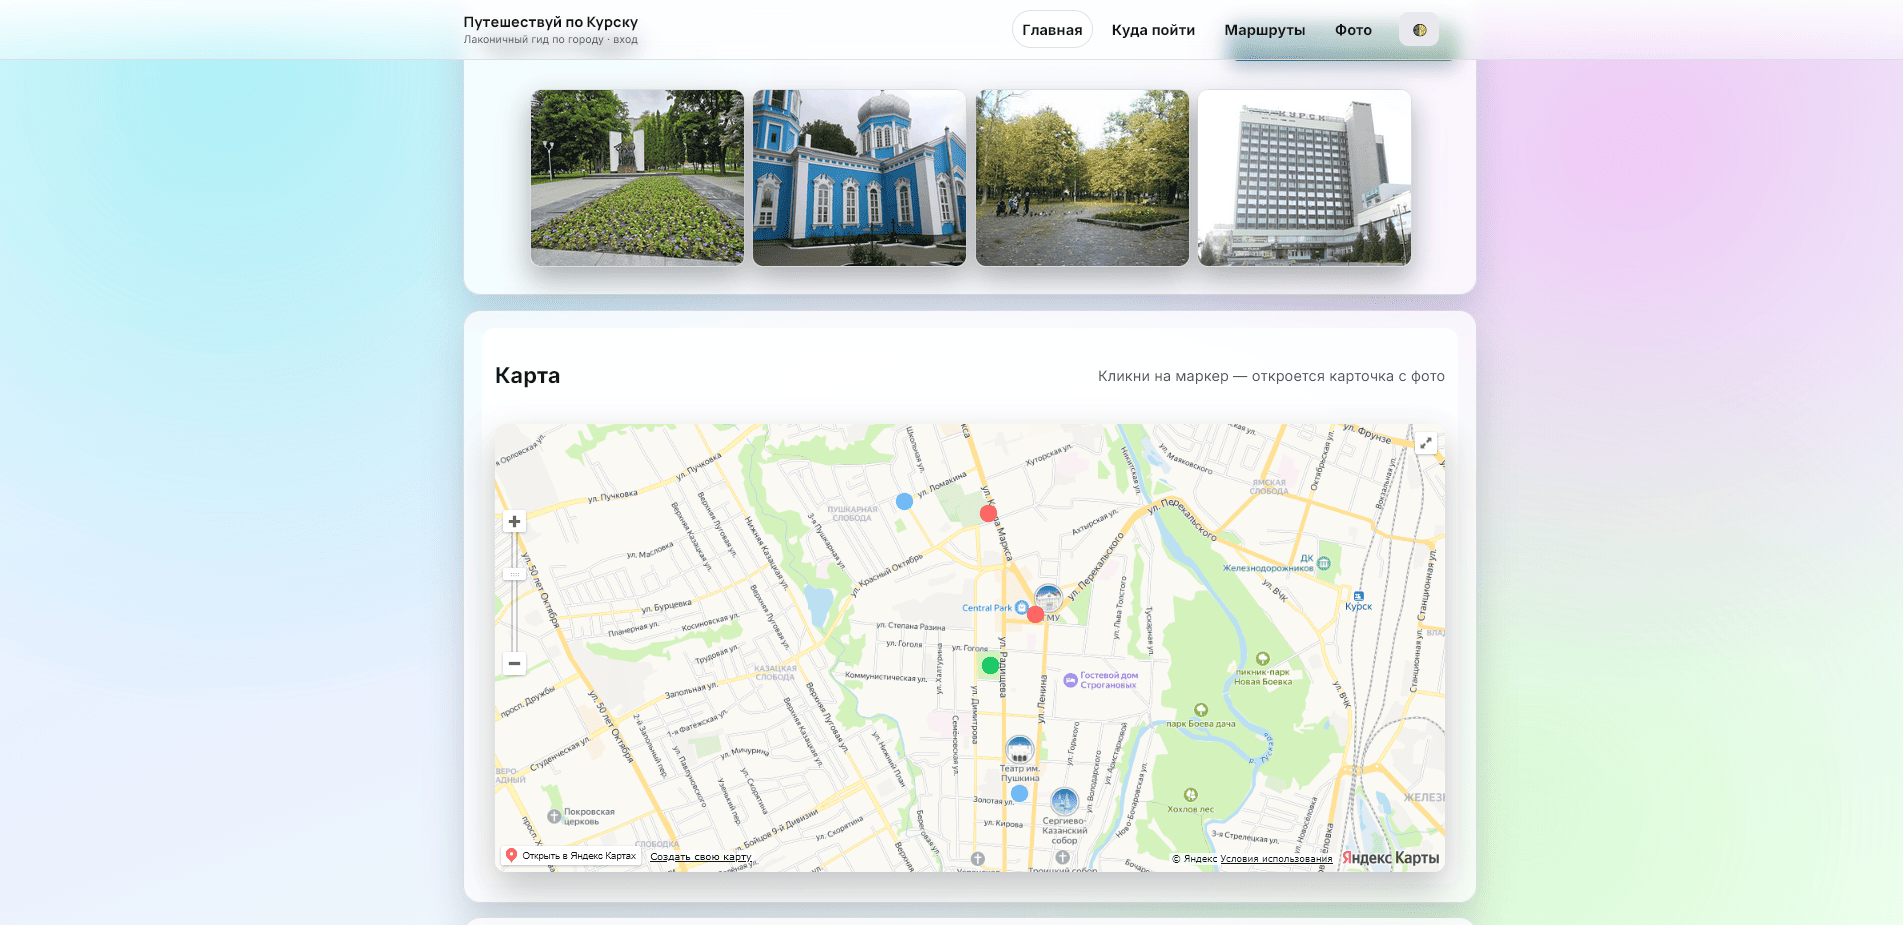
\includegraphics[width=0.9\linewidth]{images/ts-01}
	\caption{Главная страница с картой и маркерами (ТС-01)}
	\label{fig:ts-01}
\end{figure}

\subsubsection{TC-02. Фильтрация списка мест по категории}

\textbf{Предусловие:} открыта страница «Куда пойти» (\texttt{places.html}). В системе есть места разных категорий.

\textbf{Шаги:}
\begin{enumerate}
	\item В панели фильтров нажать кнопку с категорией «Парк».
	\item Проверить, что в списке карточек остались только места с категорией «парк».
	\item Нажать кнопку «Все».
	\item Убедиться, что снова отображаются все места.
\end{enumerate}

\textbf{Ожидаемый результат:} при выборе категории список карточек динамически обновляется без перезагрузки страницы. Фильтр применяется к текущему набору данных.

\textbf{Фактический результат:} пройден. Результат тестирования представ-
лен на рисунке~\ref{fig:ts-02}.

% Место для рисунка: страница places.html с активным фильтром

\begin{figure}[H]
	\centering
	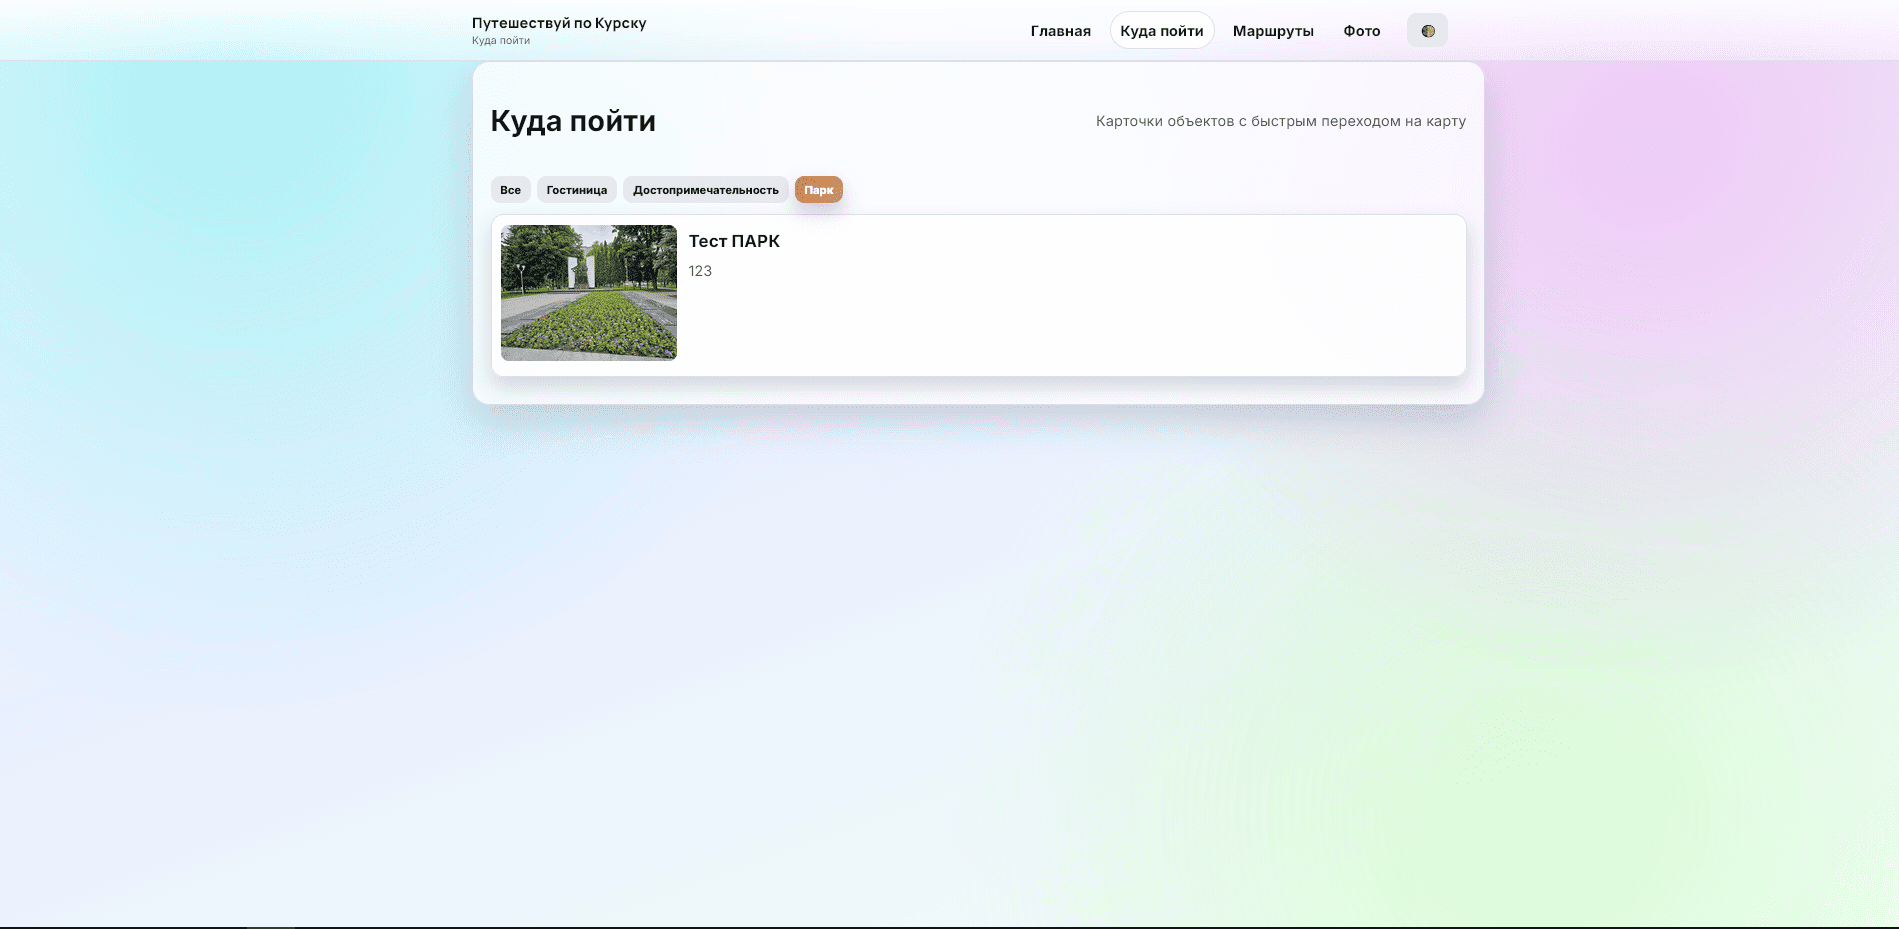
\includegraphics[width=0.9\linewidth]{images/ts-02}
	\caption{Страница «Куда пойти» с активным фильтром (ТС-02)}
	\label{fig:ts-02}
\end{figure}

\subsubsection{TC-03. Открытие карточки места и просмотр галереи}

\textbf{Предусловие:} открыта страница «Куда пойти» или главная страница с картой. Имеется место, у которого заполнены хотя бы одно изображение в галерее.

\textbf{Шаги:}
\begin{enumerate}
	\item Кликнуть по карточке места (или по маркеру на карте).
	\item В модальном окне проверить отображение названия, категории, описания, адреса, телефона, сайта.
	\item Пролистать до блока «Галерея» — увидеть миниатюры изображений.
\end{enumerate}

\textbf{Ожидаемый результат:} модальное окно содержит всю информацию об объекте. Галерея отображает до 10 изображений. Если галерея пуста, блок скрывается.

\textbf{Фактический результат:} пройден. Результат тестирования представ-
лен на рисунке~\ref{fig:ts-03}.

% Место для рисунка: модальное окно с карточкой места

\begin{figure}[H]
	\centering
	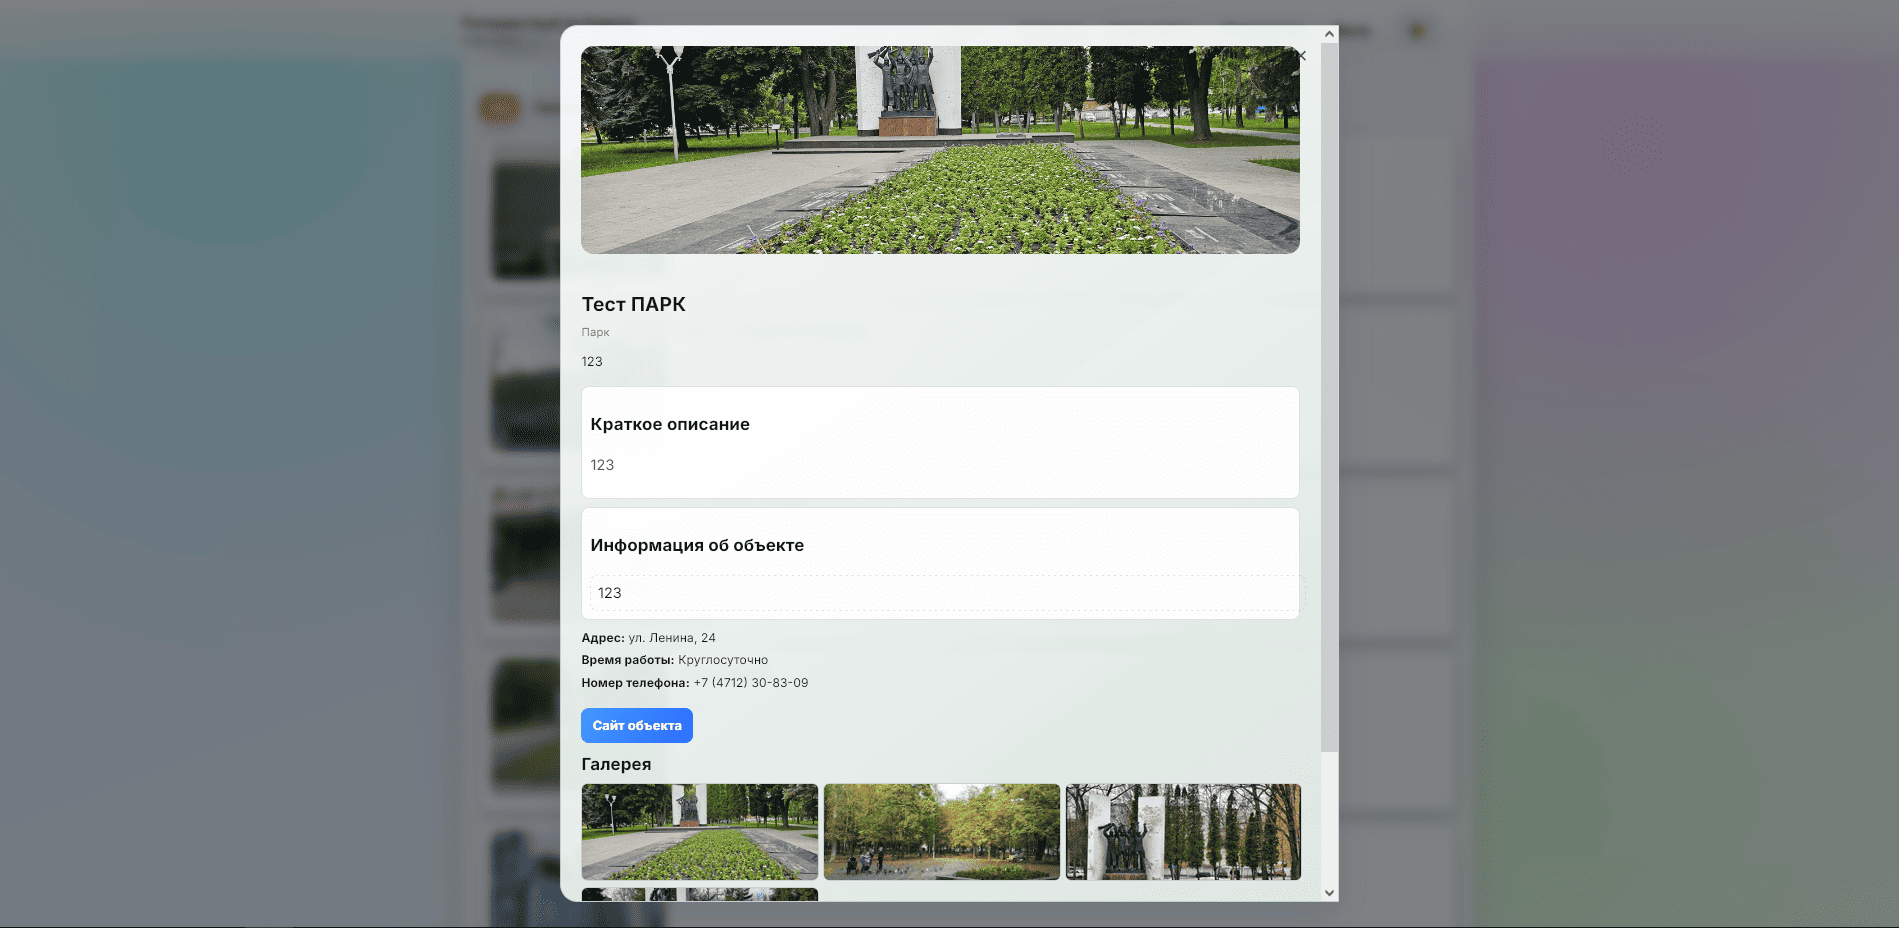
\includegraphics[width=0.9\linewidth]{images/ts-03}
	\caption{Модальное окно с карточкой места (ТС-03)}
	\label{fig:ts-03}
\end{figure}

\subsubsection{TC-04. Переход от карточки места к карте}

\textbf{Предусловие:} открыта карточка любого места (модальное окно).

\textbf{Шаги:}
\begin{enumerate}
	\item В карточке места найти кнопку «Показать на карте».
	\item Нажать на неё.
	\item Происходит переход на главную страницу (или страницу с картой), карта центрируется на выбранном месте, маркер подсвечивается.
\end{enumerate}

\textbf{Ожидаемый результат:} карта плавно перемещается к координатам места, открывается его краткая карточка (или всплывающая подсказка).

\textbf{Фактический результат:} пройден. Результат тестирования представ-
лен на рисунке~\ref{fig:ts-04}.

% Место для рисунка: карта с центрированием на месте

\begin{figure}[H]
	\centering
	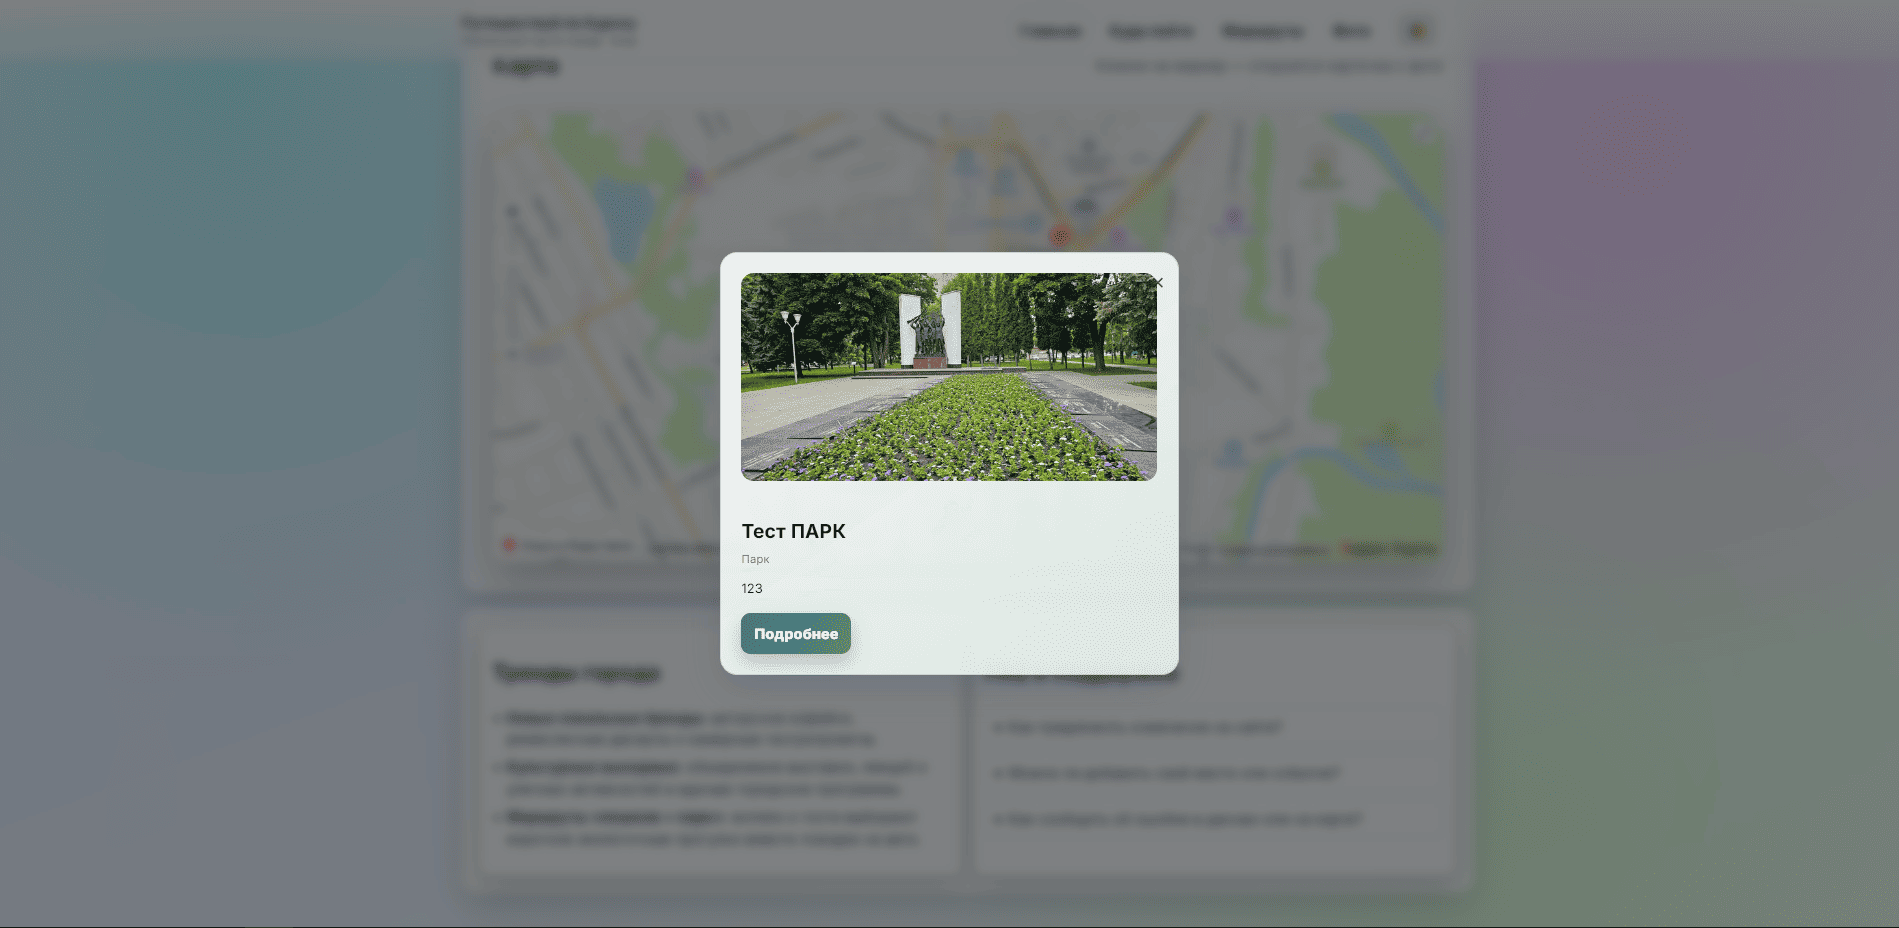
\includegraphics[width=0.9\linewidth]{images/ts-04}
	\caption{Краткая карточка объекта (ТС-04)}
	\label{fig:ts-04}
\end{figure}

\subsubsection{TC-05. Добавление нового места через админ-панель}

\textbf{Предусловие:} открыта страница администрирования.

\textbf{Шаги:}
\begin{enumerate}
	\item Заполнить форму: название «Тестовое место», выбрать категорию, указать широту и долготу, заполнить краткое описание, указать URL главного фото.
	\item По желанию добавить несколько URL в галерею (каждый с новой строки).
	\item Установить флаг «Опубликовать».
	\item Нажать «Сохранить объект».
	\item Проверить, что объект появился в таблице «Список объектов».
\end{enumerate}

\textbf{Ожидаемый результат:} объект добавляется в базу данных, отображается в админ-списке. На странице «Куда пойти» новое место видно в каталоге. На карте появляется соответствующий маркер.

\textbf{Фактический результат:} пройден. Результат тестирования представ-
лен на рисунке~\ref{fig:ts-05}.

% Место для рисунка: форма добавления места в админке

\begin{figure}[H]
	\centering
	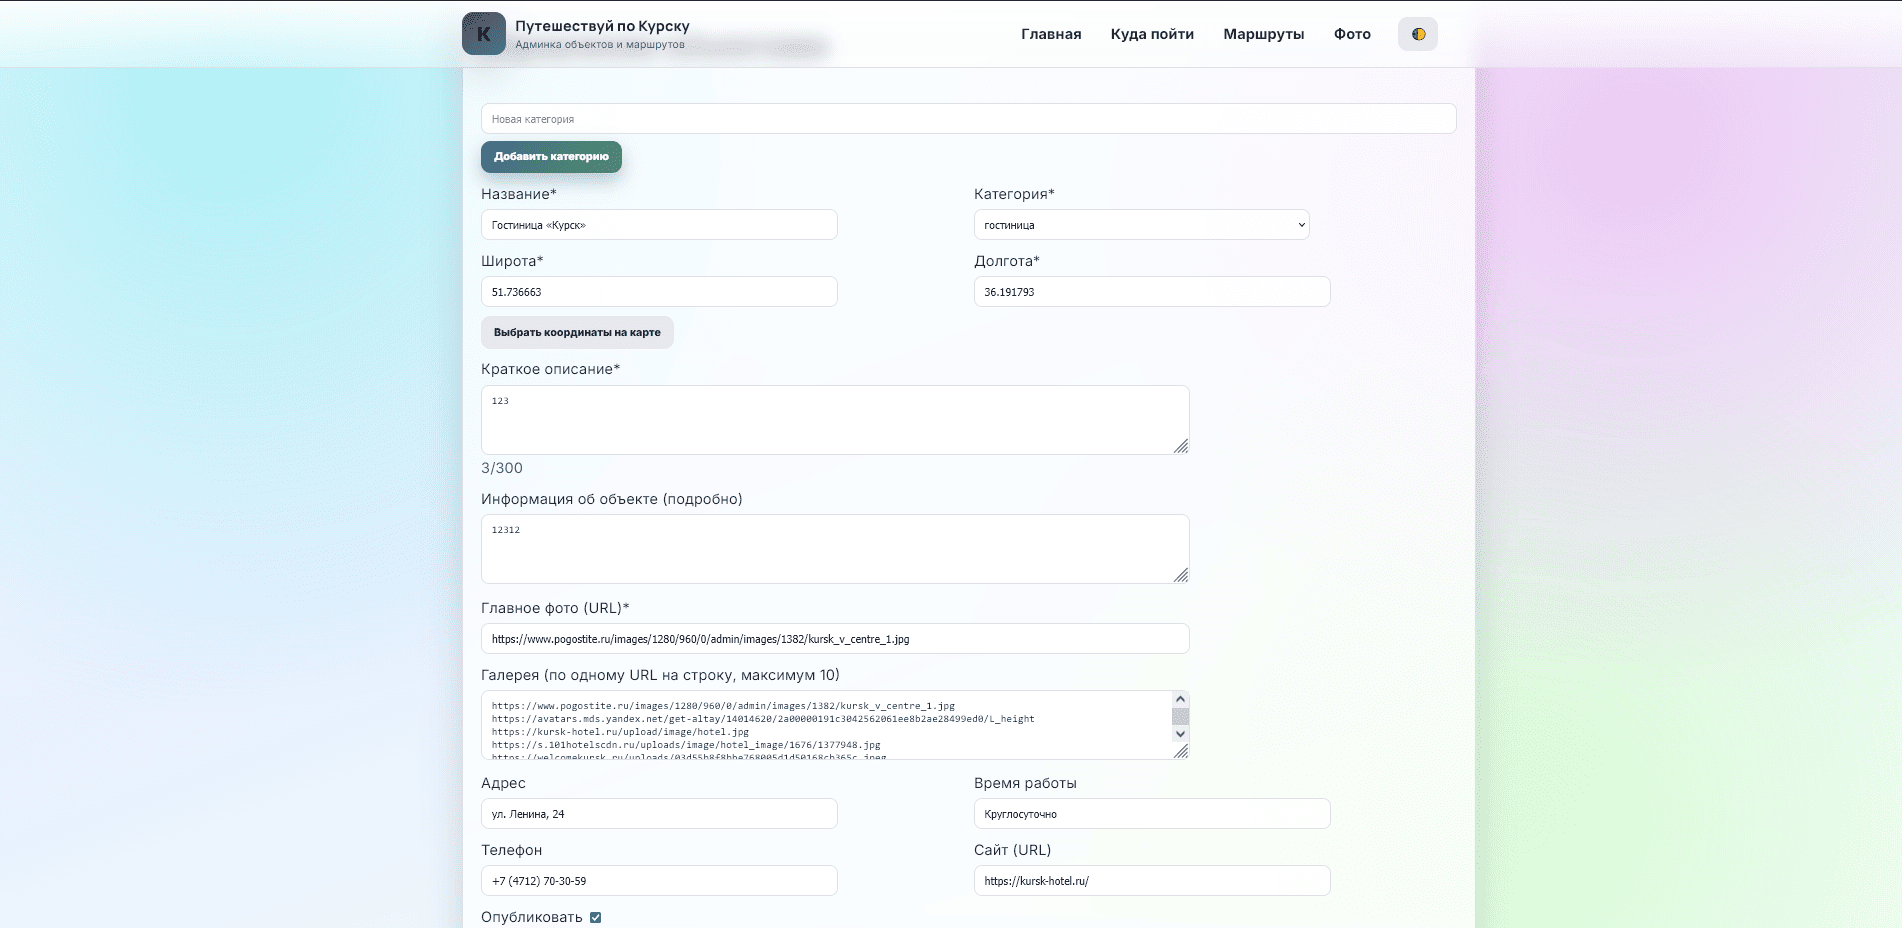
\includegraphics[width=0.9\linewidth]{images/ts-05}
	\caption{Форма добавления места (ТС-05)}
	\label{fig:ts-05}
\end{figure}

\subsubsection{TC-06. Редактирование существующего места}

\textbf{Предусловие:} в системе есть хотя бы одно место. Открыта админ-панель.

\textbf{Шаги:}
\begin{enumerate}
	\item В таблице «Список объектов» нажать кнопку «Редактировать» у выбранного места.
	\item Изменить название или описание.
	\item Нажать «Обновить объект».
\end{enumerate}

\textbf{Ожидаемый результат:} данные места обновляются в базе. На странице «Куда пойти» отображается актуальная информация.

\textbf{Фактический результат:} пройден. Результат тестирования представ-
лен на рисунке~\ref{fig:ts-06}.

% Место для рисунка: форма редактирования места

\begin{figure}[H]
	\centering
	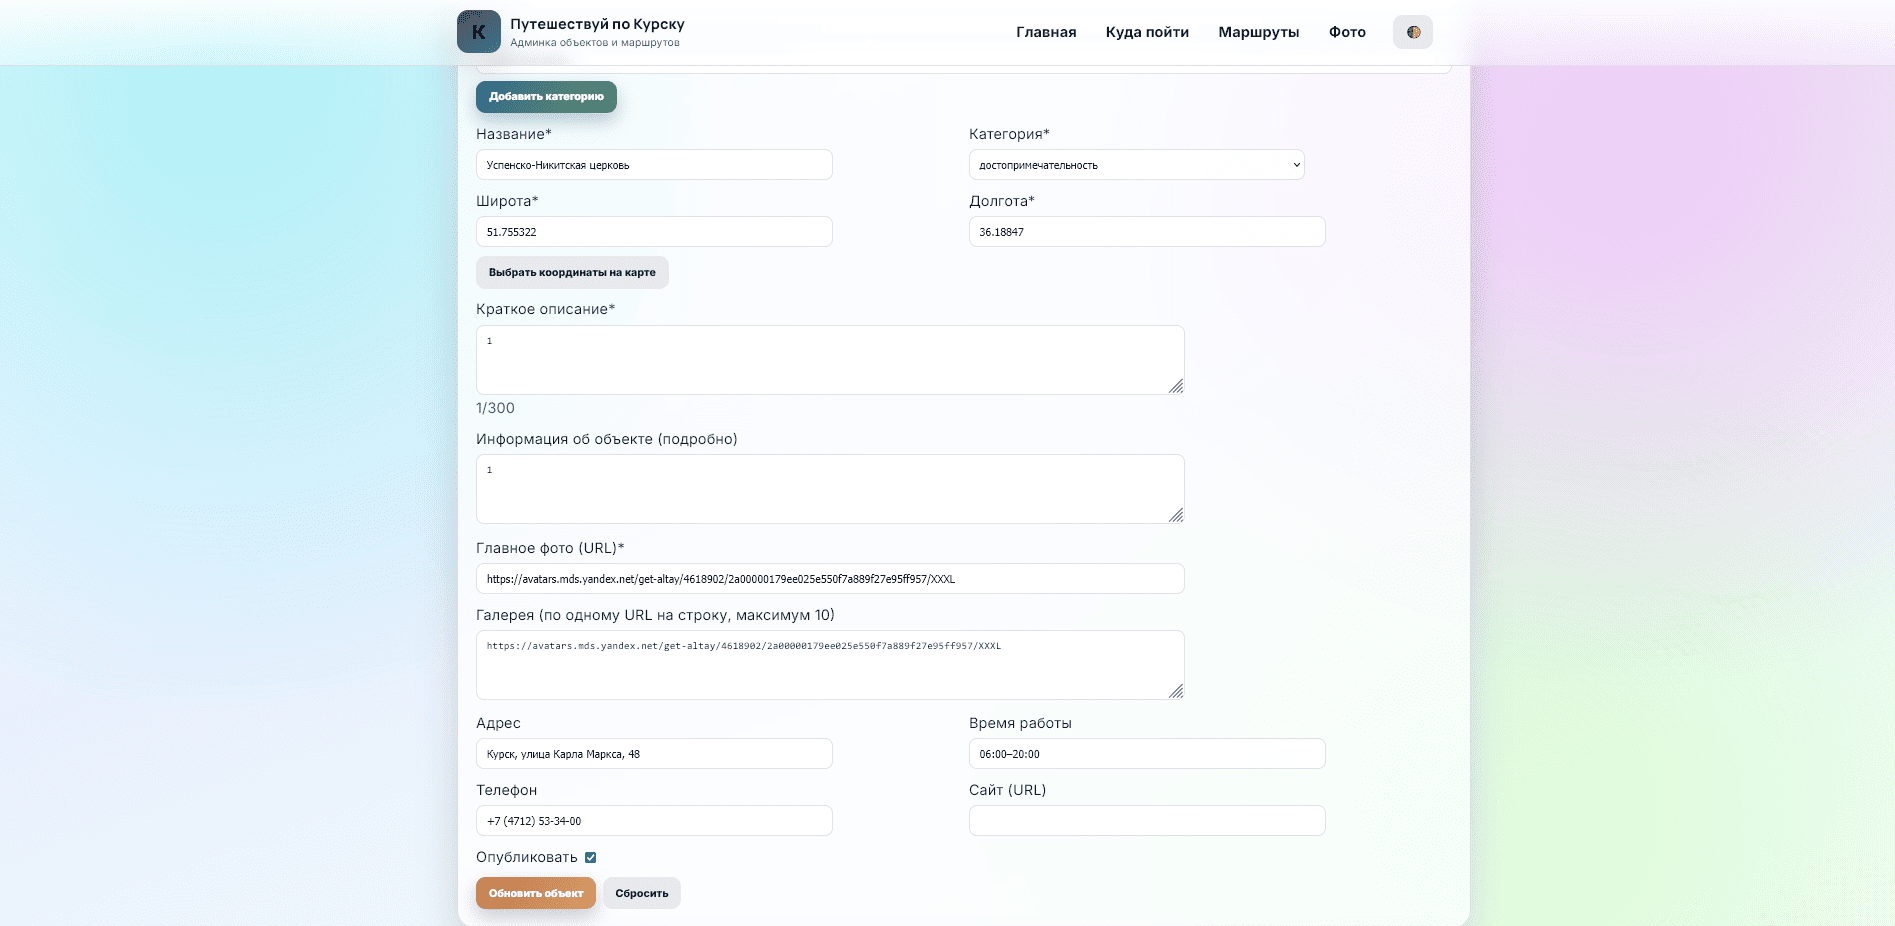
\includegraphics[width=0.9\linewidth]{images/ts-06}
	\caption{Форма редактирования места (ТС-06)}
	\label{fig:ts-06}
\end{figure}

\subsubsection{TC-07. Добавление новой категории}

\textbf{Предусловие:} открыта админ-панель.

\textbf{Шаги:}
\begin{enumerate}
	\item В поле «Новая категория» ввести, например, «Театр».
	\item Нажать кнопку «Добавить категорию».
	\item В выпадающем списке категорий (в форме объекта) появится новая категория.
\end{enumerate}

\textbf{Ожидаемый результат:} категория сохраняется в таблице \texttt{categories} и доступна для выбора при добавлении/редактировании мест.

\textbf{Фактический результат:} пройден. Результат тестирования представ-
лен на рисунке~\ref{fig:ts-07}.

% Место для рисунка: добавление категории

\begin{figure}[H]
	\centering
	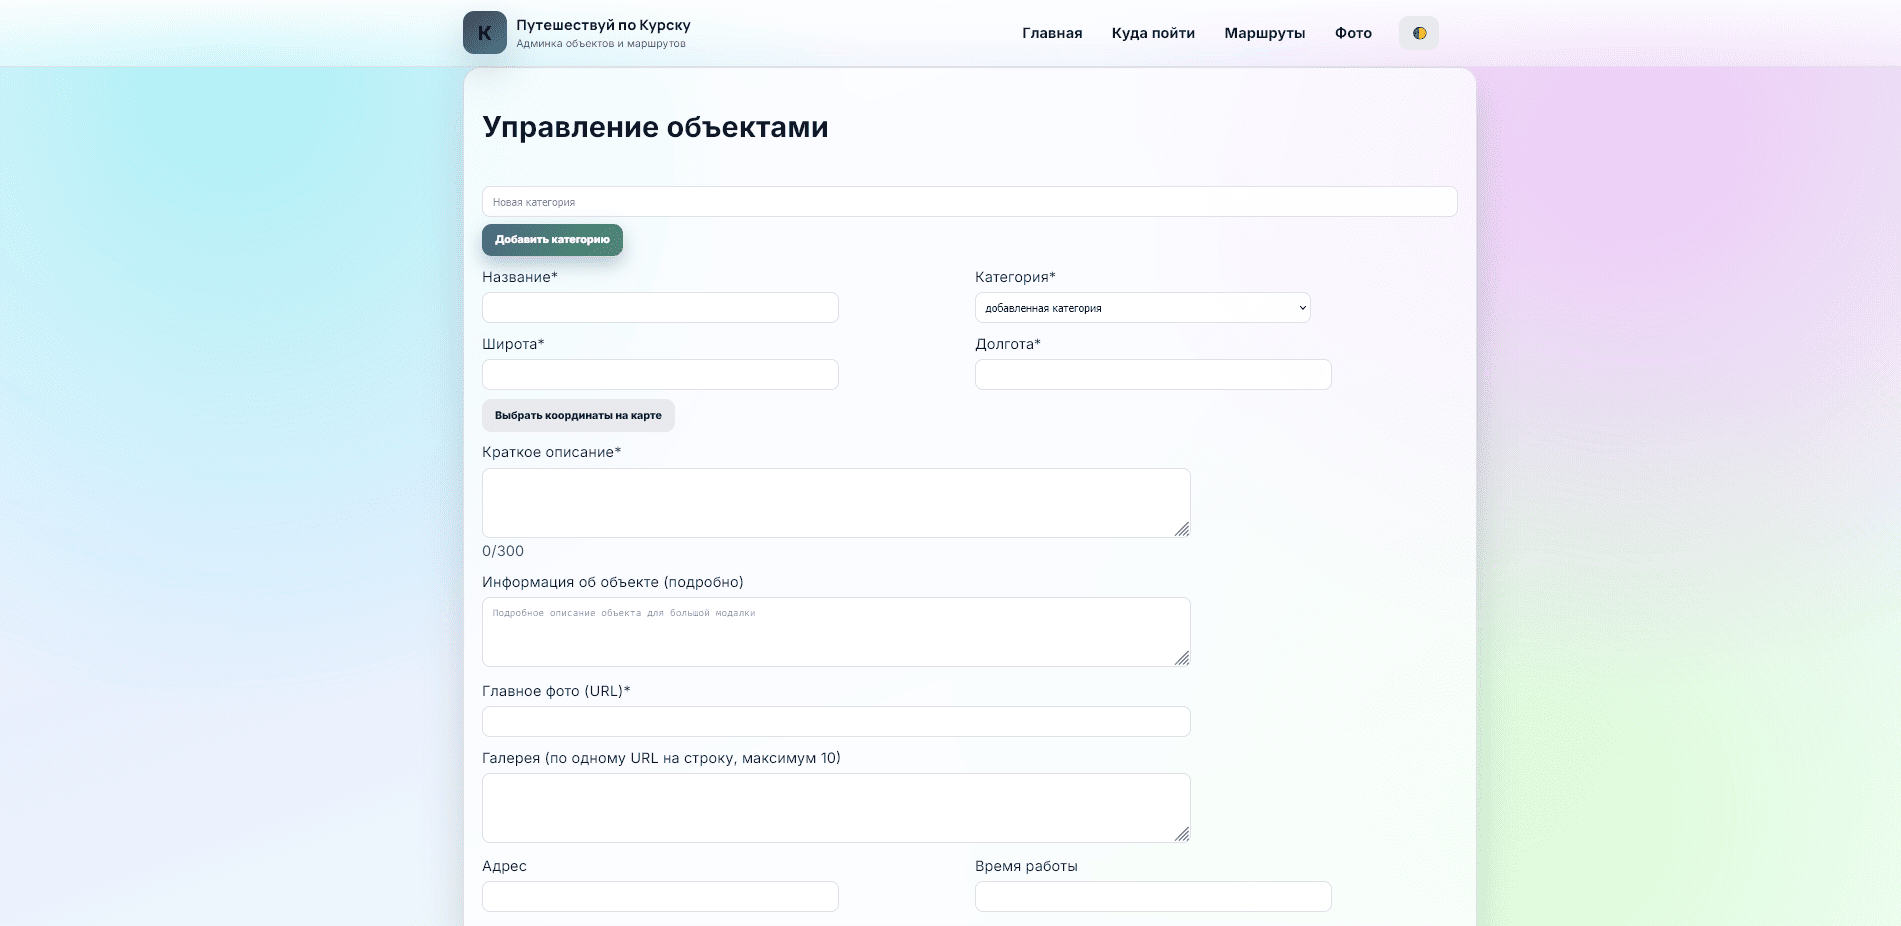
\includegraphics[width=0.9\linewidth]{images/ts-07}
	\caption{Добавленная категория (ТС-07)}
	\label{fig:ts-07}
\end{figure}

\subsubsection{TC-08. Создание маршрута (выбор точек, порядок)}

\textbf{Предусловие:} в системе существует минимум два места. Открыта админ-панель, раздел управления маршрутами.

\textbf{Шаги:}
\begin{enumerate}
	\item Заполнить название маршрута, краткое описание.
	\item В блоке «Точки маршрута» выбрать место из выпадающего списка и нажать «Добавить точку». Повторить для второго и третьего места.
	\item Изменить порядок точек кнопками «↑» и «↓».
	\item Установить флаг «Опубликовать».
	\item Нажать «Сохранить маршрут».
\end{enumerate}

\textbf{Ожидаемый результат:} маршрут сохраняется в БД. Точки сохраняются в таблице \texttt{route\_points} с правильными позициями. При попытке сохранить маршрут менее чем с двумя точками — ошибка валидации.

\textbf{Фактический результат:} пройден. Результат тестирования представ-
лен на рисунке~\ref{fig:ts-08}.

% Место для рисунка: форма создания маршрута

\begin{figure}[H]
	\centering
	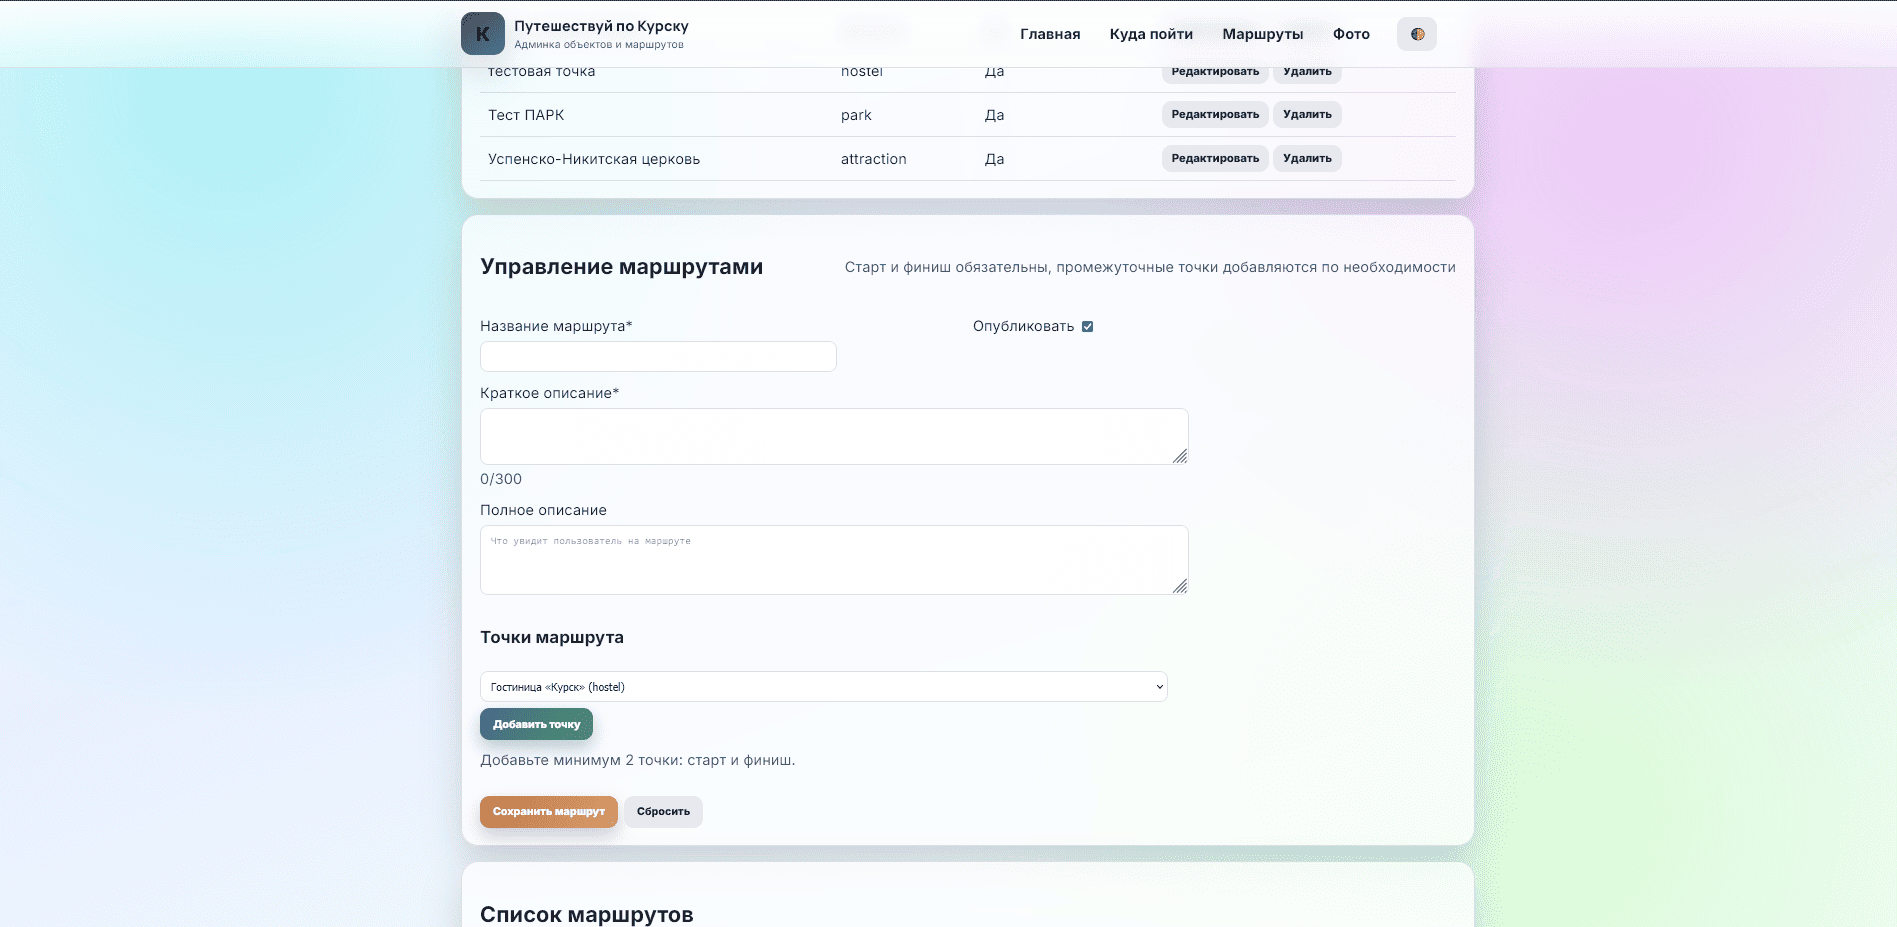
\includegraphics[width=0.9\linewidth]{images/ts-08}
	\caption{Форма создания маршрута (ТС-08)}
	\label{fig:ts-08}
\end{figure}

\subsubsection{TC-09. Редактирование маршрута}

\textbf{Предусловие:} в системе есть хотя бы один маршрут.

\textbf{Шаги:}
\begin{enumerate}
	\item В таблице «Список маршрутов» нажать «Редактировать».
	\item Изменить название, описание или состав точек.
	\item Сохранить изменения.
\end{enumerate}

\textbf{Ожидаемый результат:} маршрут обновляется в БД. При просмотре на странице «Маршруты» отображаются актуальные данные.

\textbf{Фактический результат:} пройден. Результат тестирования представ-
лен на рисунке~\ref{fig:ts-09}.

% Место для рисунка: редактирование маршрута

\begin{figure}[H]
	\centering
	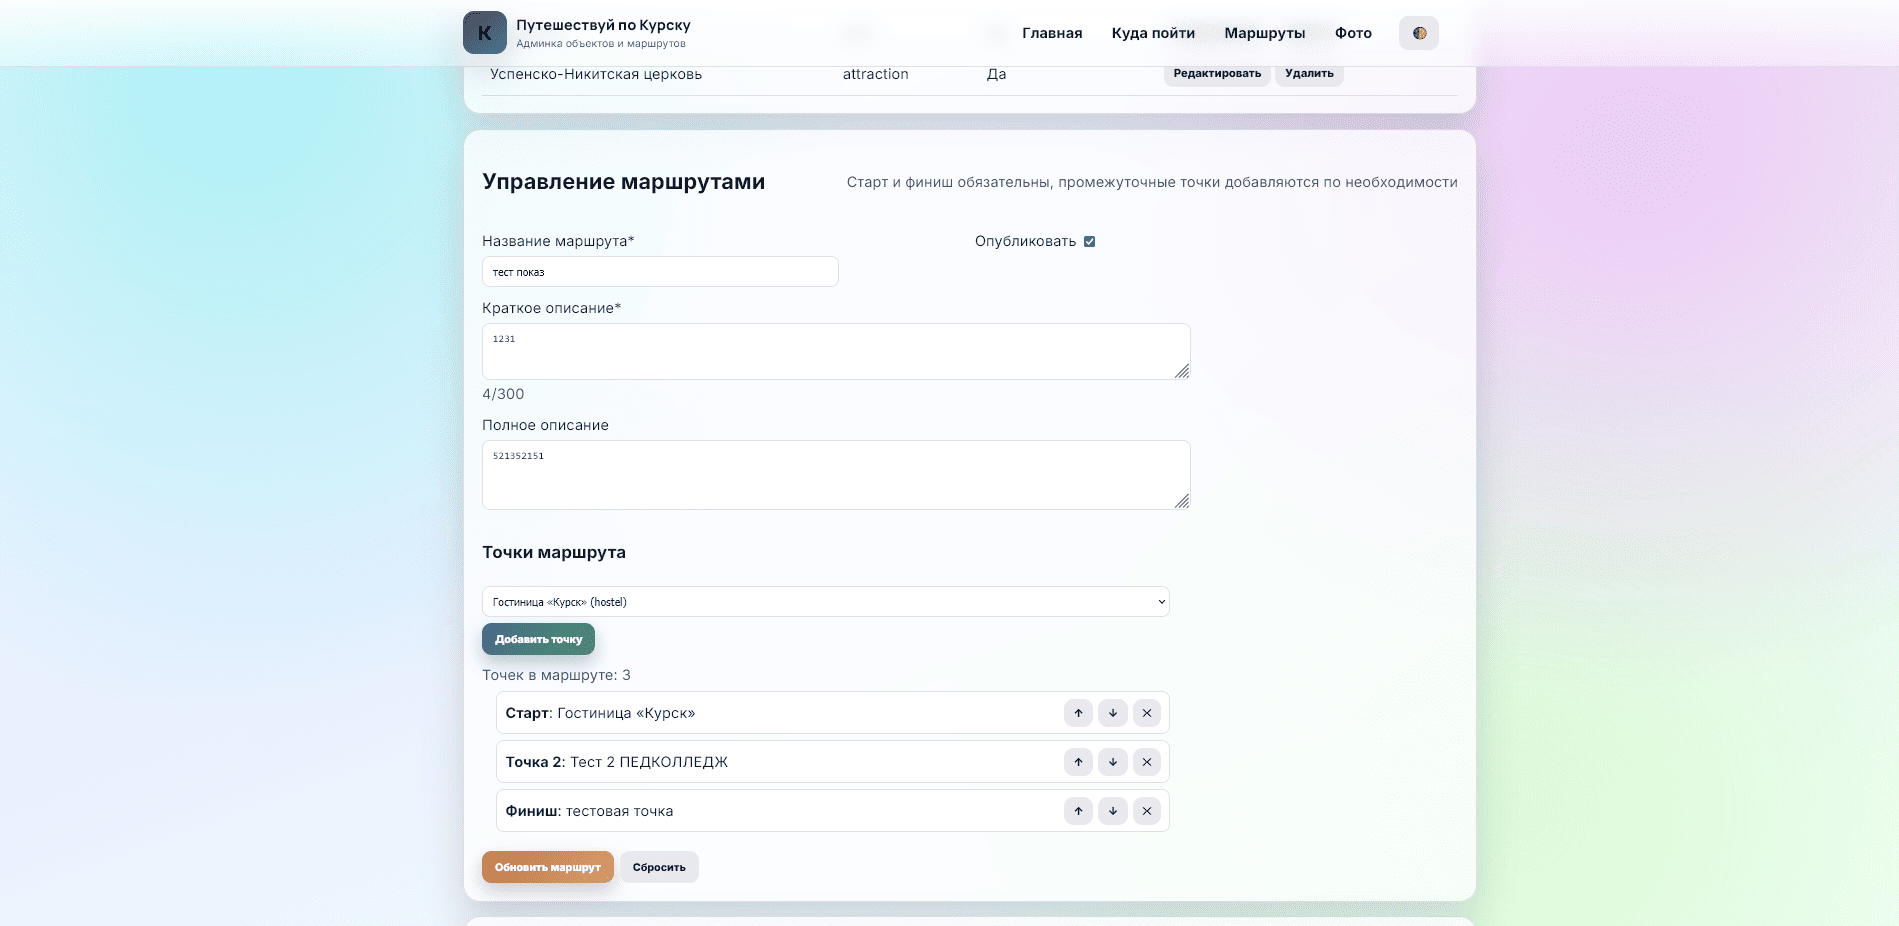
\includegraphics[width=0.9\linewidth]{images/ts-09}
	\caption{Форма редактирования маршрута (ТС-09)}
	\label{fig:ts-09}
\end{figure}

\subsubsection{TC-10. Просмотр маршрута на карте (пешеходная прокладка)}

\textbf{Предусловие:} опубликован маршрут с корректными координатами точек (минимум две).

\textbf{Шаги:}
\begin{enumerate}
	\item Перейти на страницу «Маршруты» (\texttt{routes.html}).
	\item Нажать кнопку «Открыть маршрут» на карточке любого маршрута.
	\item В модальном окне проверить описание и список точек.
	\item Дождаться загрузки карты в нижней части модального окна.
\end{enumerate}

\textbf{Ожидаемый результат:} на карте построена линия пешеходного маршрута с использованием \texttt{ymaps.multiRouter}. Отображаются старт, финиш и промежуточные точки.

\textbf{Фактический результат:} пройден. Результат тестирования представ-
лен на рисунке~\ref{fig:ts-10}.

% Место для рисунка: модальное окно с маршрутом на карте

\begin{figure}[H]
	\centering
	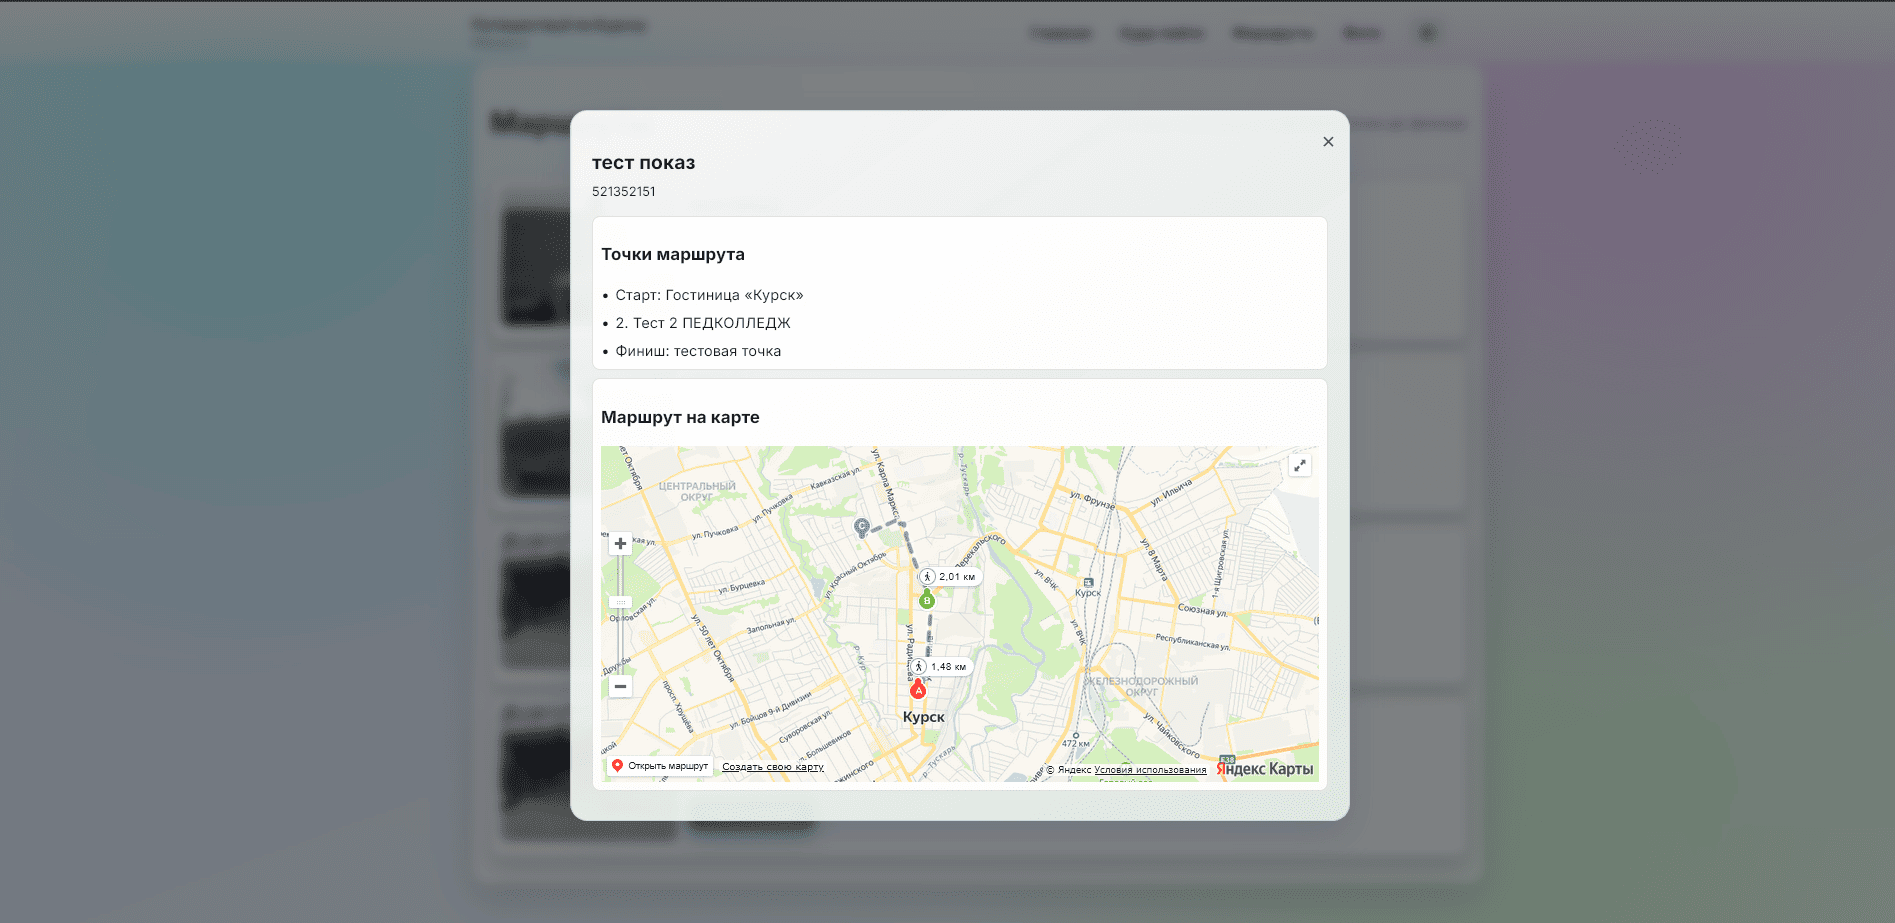
\includegraphics[width=0.9\linewidth]{images/ts-10}
	\caption{Модальное окно маршрута (ТС-10)}
	\label{fig:ts-10}
\end{figure}

\subsubsection{TC-11. Отображение фотогалереи всех мест}

\textbf{Предусловие:} в системе есть несколько мест с заполненными главными фото и галереями.

\textbf{Шаги:}
\begin{enumerate}
	\item Перейти на страницу «Фото».
	\item Просмотреть сетку изображений.
\end{enumerate}

\textbf{Ожидаемый результат:} сетка содержит все уникальные изображения (главные фото + галереи) из всех опубликованных мест. Порядок может быть случайным.

\textbf{Фактический результат:} пройден. Результат тестирования представ-
лен на рисунке~\ref{fig:ts-11}.

% Место для рисунка: страница photos.html

\begin{figure}[H]
	\centering
	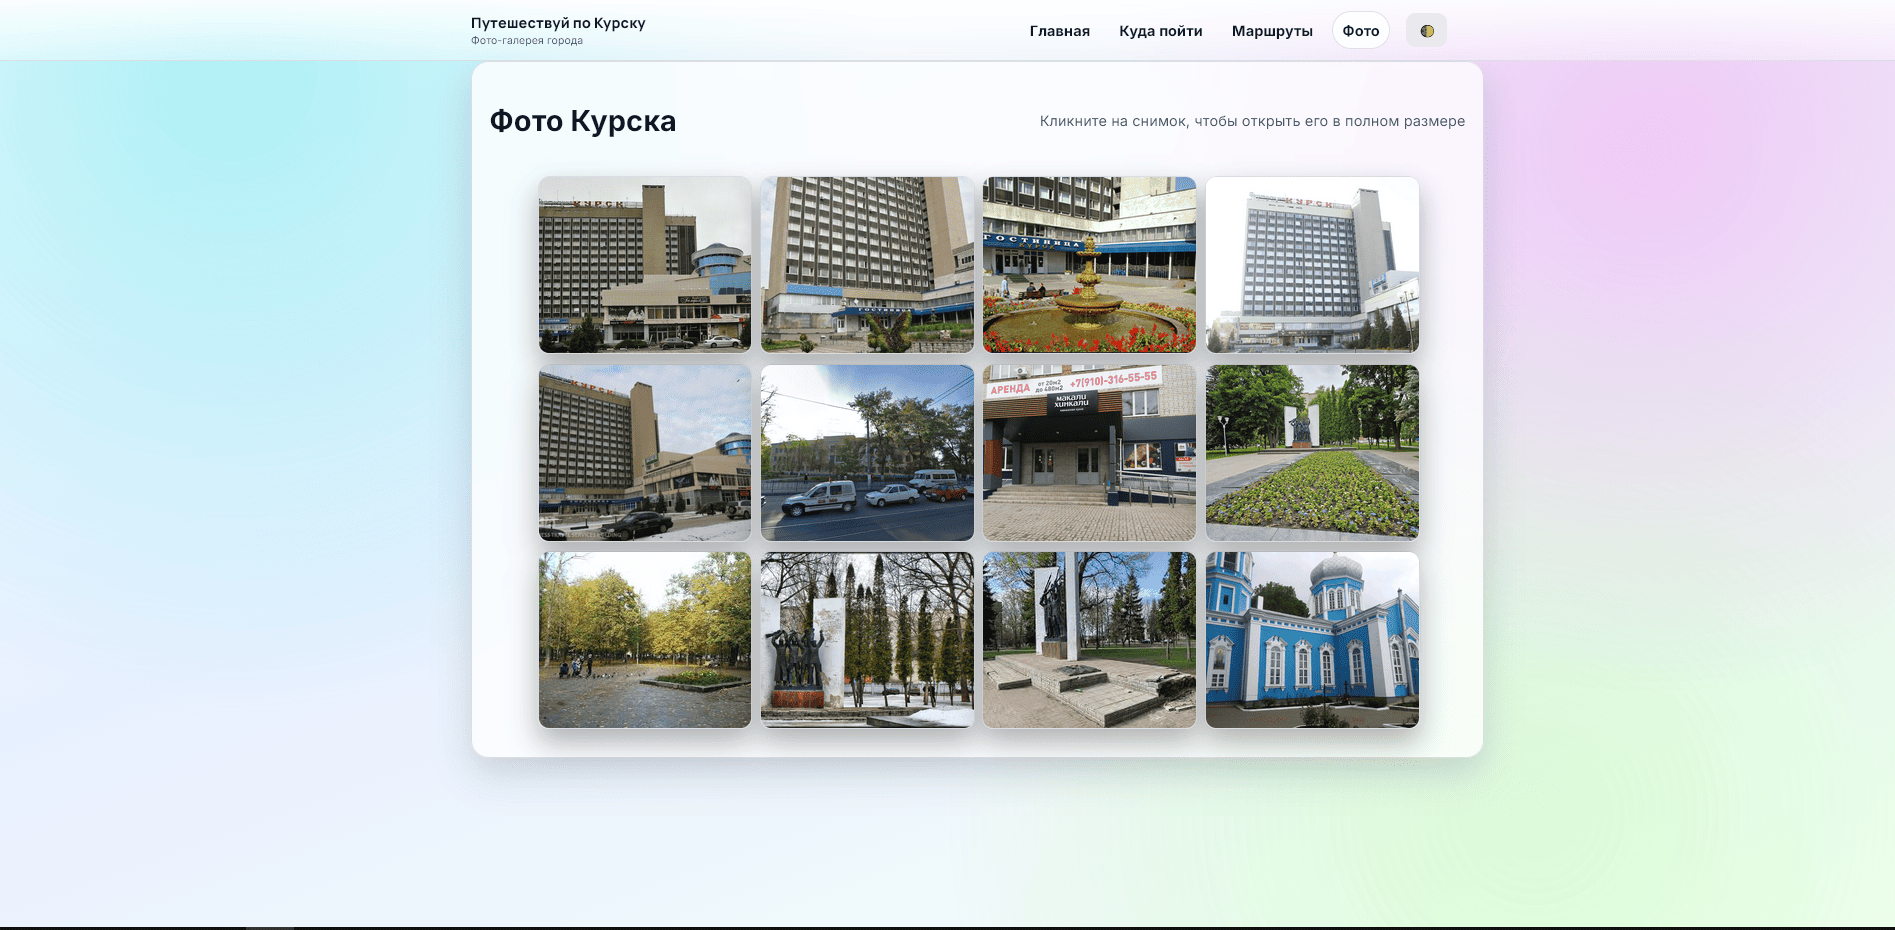
\includegraphics[width=0.9\linewidth]{images/ts-11}
	\caption{Страница «Фото» (ТС-11)}
	\label{fig:ts-11}
\end{figure}

\subsubsection{TC-12. Выбор координат объекта на карте в админке}

\textbf{Предусловие:} открыта форма добавления/редактирования места в админ-панели.

\textbf{Шаги:}
\begin{enumerate}
	\item Нажать кнопку «Выбрать координаты на карте».
	\item В открывшемся модальном окне дождаться загрузки карты.
	\item Кликнуть левой кнопкой мыши в любом месте карты.
	\item В диалоговом окне подтверждения нажать «OK».
\end{enumerate}

\textbf{Ожидаемый результат:} поля «Широта» и «Долгота» в форме автоматически заполняются выбранными координатами (6 знаков после запятой). Модальное окно закрывается.

\textbf{Фактический результат:} пройден. Результат тестирования представ-
лен на рисунке~\ref{fig:ts-14}.

% Место для рисунка: модальное окно выбора координат

\begin{figure}[H]
	\centering
	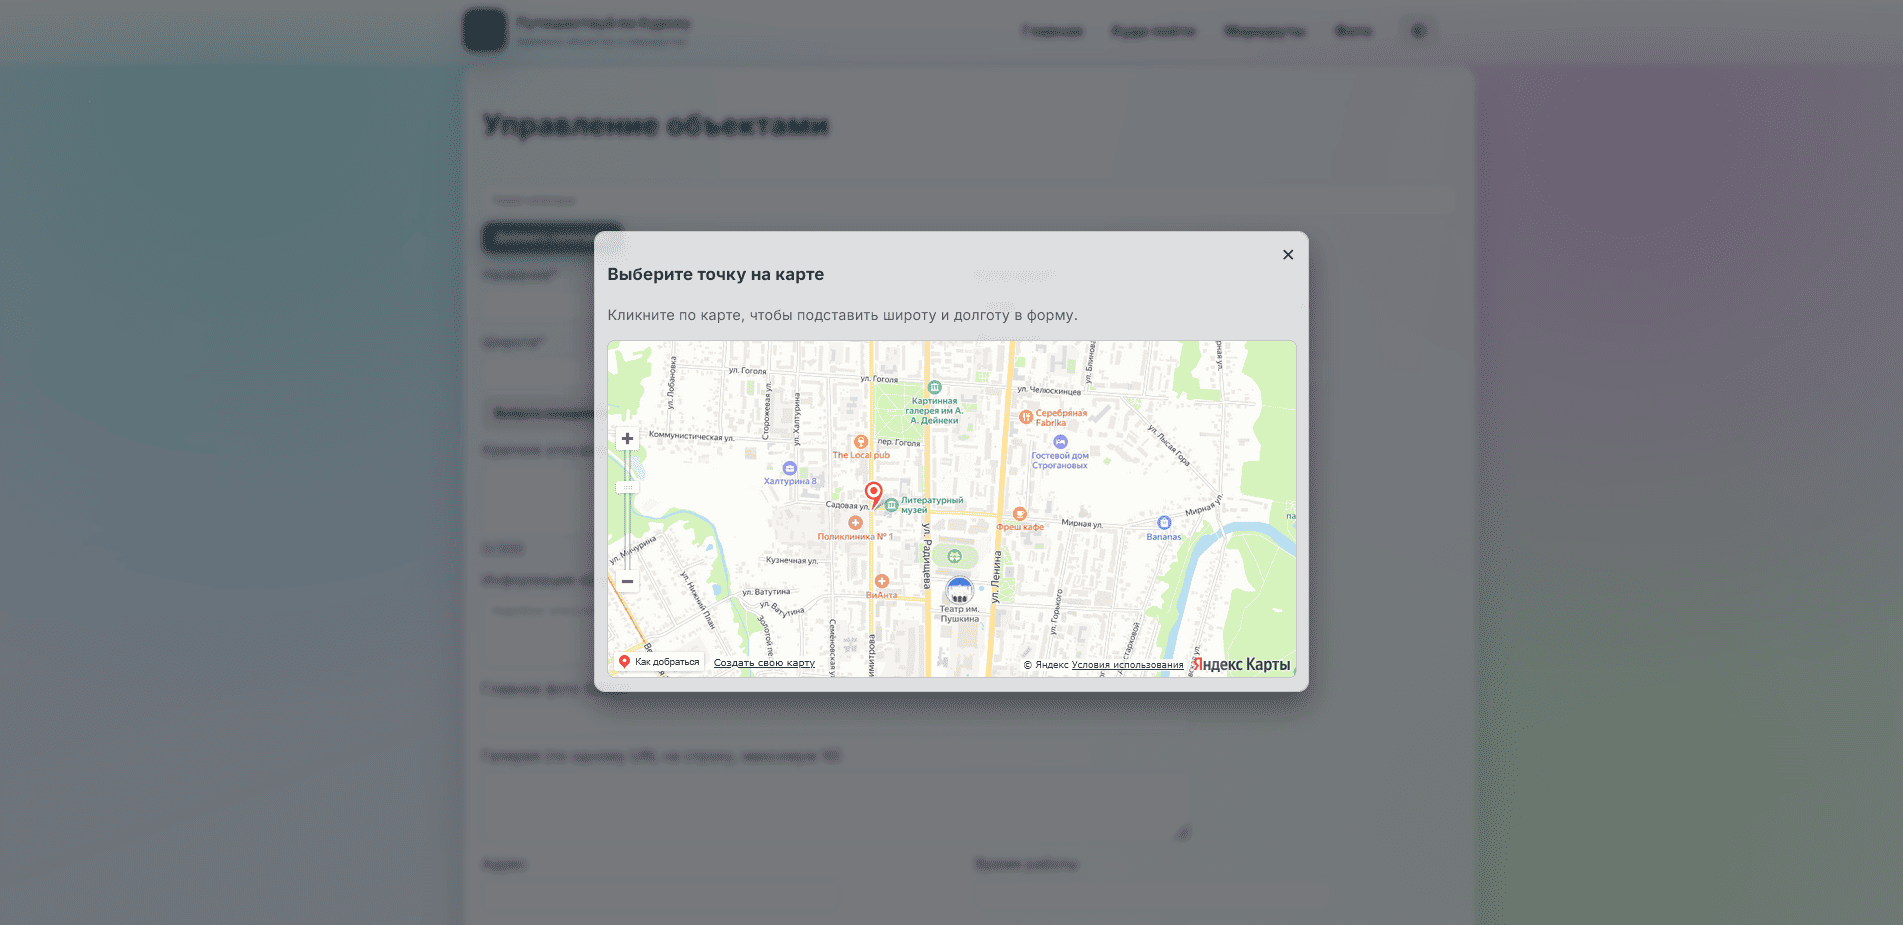
\includegraphics[width=0.9\linewidth]{images/ts-14}
	\caption{Модальное окно выбора координат (ТС-12)}
	\label{fig:ts-14}
\end{figure}

\subsubsection{Нефункциональное тестирование}

Проверены нефункциональные требования (разделы 2.6–2.8 ТЗ):

\begin{enumerate}
	\item Быстродействие: загрузка главной страницы с картой и 50 маркерами — не более 2 с. Фильтрация мест — мгновенно (< 100 мс). Сохранение места/маршрута — < 500 мс.
	\item Корректность логирования: ошибки API логируются в консоли сервера, клиенту возвращается JSON с полем \texttt{error}.
	\item Совместимость с браузерами: тестирование в Chrome, Firefox, Yandex Browser, Edge — все функции работают корректно.
	\item Надёжность: при разрыве соединения с БД сервер возвращает HTTP 500. Транзакционное сохранение маршрута гарантирует целостность.
\end{enumerate}

Все нефункциональные требования выполнены.

\subsubsection{Вывод по результатам тестирования}

В ходе системного тестирования успешно проверены все функциональные и нефункциональные требования. Веб-приложение работает стабильно, интерфейс интуитивно понятен, все сценарии использования выполняются корректно. Система готова к эксплуатации.